\documentclass[11pt]{article}

\usepackage{csquotes}
\usepackage[hidelinks]{hyperref}
\usepackage{setspace}
\usepackage{fancyhdr}
\usepackage{xcolor}
\usepackage{soul}
\usepackage{amsmath}
\usepackage{amssymb}
\usepackage{mathtools}
\usepackage{braket}
\usepackage{colonequals}
\usepackage{amsopn}
\usepackage[version=4]{mhchem}
\usepackage{gensymb}
\usepackage{graphicx}
\usepackage{caption}
\usepackage{wrapfig}
\usepackage{tabularx}
\usepackage{booktabs}
\usepackage{multirow}
\usepackage{tikz}
\usepackage{natbib}

\title{Welcome to Texpile}
\author{A live tutorial project}
\date{\today}

\begin{document}

\maketitle

\section{What is Texpile}

Texpile is both a visual and a non-visual, fully offline LaTeX editor. This document covers the
basics to get you started.

\section{Switching between visual and non-visual}

In the top right corner you can see a toggle between the visual and non-visual (Source) editor:

\begin{figure}[h]
	\centering
	
\includegraphics{images/visual-source-toggle.png}
\end{figure}

The visual editor parses your current LaTeX code and renders it live. In most cases the visual
editor will feel perfect, but if your document is complicated, sometimes it'll leave raw LaTeX
floating around inline instead of rendering it.

The visual editor also supports advanced features like table cell merging and pasting images
directly. Feel free to try them in this document.

\section{This is a multi-file project}

Texpile supports multiple files and autocomplete (intellisense). It also supports git, with a
Source Control panel and diff views. Explore more of these from the left sidebar.

\section{Compiling and formatting}

Compiling turns this source into a PDF using your own LaTeX distribution. Texpile does not bundle
any LaTeX distribution.

If you don't have a local TeX distribution installed, you can install one of these:
\href{https://tug.org/texlive/}{TeX Live} (Linux, macOS, Windows) or
\href{https://miktex.org/}{MiKTeX} (Windows).

Texpile's default compile command is:
\begin{verbatim}
latexmk -lualatex -interaction=nonstopmode -file-line-error
        -synctex=1 -output-directory=output {main}
\end{verbatim}
\texttt{\{main\}} expands to this project's main file. \texttt{-synctex=1} is what lets you
double-click inside the compiled PDF to jump to the matching source line, and back.
\texttt{-output-directory=output} keeps aux/log files out of your project folder.

When you install MacTeX, it's supposed to symlink its binaries into \texttt{/Library/TeX/texbin}
and add that to your PATH, but this step can fail to complete, or need a fresh Terminal window to
take effect, so \texttt{latexmk} can come back ``not found'' even in Terminal right after
installing. If that happens, re-run the MacTeX installer, or open TeX Live Utility and use its
repair option.

If you'd rather use pdflatex or xelatex, or need any other custom command, open the Terminal
menu and choose \textbf{Configure compile command\ldots}.

Before compiling a multi-file project, right-click its main .tex file in the file tree on the left
and choose \textbf{Set as main file}. Once set, you'll see a star next to it:

\begin{figure}[h]
	\centering
	
\includegraphics{images/main-file-star.png}
\end{figure}

Formatting your source doesn't have to be manual either: the Format menu's \textbf{Format
document} command reindents your file with \texttt{latexindent}, without changing what it renders.
Try it below: \texttt{math-and-figures.tex} is deliberately messy, so switch to Source mode there
and run Format document to watch it clean up automatically.

\section{Formatting and spell-check}

Formatting shortcuts work the same in both views: \textbf{Ctrl+B} bold, \textbf{Ctrl+I} italic,
\textbf{Ctrl+U} underline, \textbf{Ctrl+\`{}} monospace, plus the toolbar buttons above. Select some
text here and try one.

Spell-check runs locally, no network involved, and is off by default. Turn on \textbf{Check
spelling \& grammar} from the Spelling menu, and the misspelled wrod right here gets flagged; click
it for a suggestion.

\subsection{Lists}

\begin{itemize}
	\item Press Enter at the end of an item to add another, or use the toolbar.
	\item Tab indents into a sub-list; Shift+Tab un-indents.
\end{itemize}

\subsection{Tables}

\begin{table}[h]
	\centering
	\begin{tabular}{lcc}
		\toprule
		Feature & Visual mode & Source mode \\
		\midrule
		Formatting shortcuts & Yes & Yes \\
		Autocomplete & No & Yes \\
		WYSIWYG preview & Yes & No \\
		\bottomrule
	\end{tabular}
	\caption{Click directly into any cell to edit it. Use the toolbar's table button, or right-click a cell, to add or remove rows and columns. Select two or more cells and right-click to merge them.}
\end{table}


\section{Math}

  Type \textbackslash( to start inline math and Texpile recognizes it immediately: \(E = mc^2\).
Display math gets its own line:
\[
        \int_0^\infty e^{-x^2}\,dx = \frac{\sqrt{\pi}}{2}
  \]

\section{Figures and references}

Drag an image file from your file manager straight into the editor to insert it directly; this one
      was added that way. Copy an image and paste it (Ctrl+V) works too.

\begin{figure}[h]
		\centering
	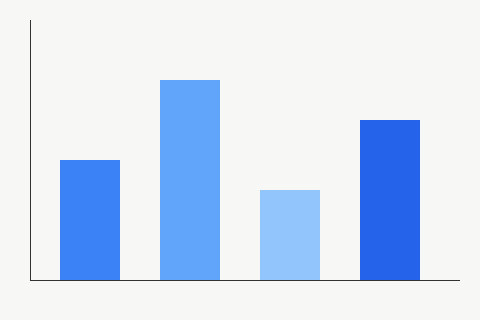
\includegraphics[width=0.6\textwidth]{images/sample.png}
			\caption{Image paths resolve relative to this folder, the same as \texttt{\textbackslash input}.}
	\label{fig:sample}
	\end{figure}

  In Source mode, typing \texttt{\textbackslash ref\{} or \texttt{\textbackslash cite\{}
autocompletes from this project's own labels and \texttt{references.bib}: see
Figure~\ref{fig:sample}, or \citep{doe2024} and \citet{smith2023} for both citation styles.


\section{Further reading}

Keyboard shortcuts and support links are under the Help menu, not here.

Texpile is open source; please report issues (and consider starring the project) at
\href{https://github.com/nullpointerexceptionkek/texpile-monorepo}{github.com/nullpointerexceptionkek/texpile-monorepo}.

\bibliography{references}
\bibliographystyle{plainnat}

\end{document}
